% !TeX spellcheck = da_DK
\subsection{Feedbackkonfiguration}
\subsubsection{Teori og design} \label{Afs_Komparator}
Jævnfør \ref{Komparatorafsnit} på side \pageref{Komparatorafsnit} anvendes en komparator til at sammenligne to inputspændinger. Komparatoren der anvendes er af typen LM311. Ved denne type placeres en $100$nF kondensator i en sammenkobling af komparatorens balanceben, for at gøre komparatoren mere præcis og undgå svingninger \cite{Instruments2015}. Der anvendes flere komparatorer, disse tilkobles ved outputtet enten en LED eller en vibrator, samt en modstand og den positive spændingsforsyning ($+V_{cc}$). I komparatorernes ikke-inverterende terminaler tilsluttes outputtet fra forrige blok, hvor inputtet i de inverterende terminaler fungerer som referencespænding, der forsynes med de beregnede tærskelværdier. Komparatorerne kan derfor have to forskellige outputs afhængig af inputspændingen. Hvis inputsignalet ligger under de beregnede tærskelværdier vil outputtet være $0V$ og LEDerne samt de to vibratorer vil ikke blive aktiveret. Er inputtet derimod over de beregnede tærskelværdier, vil outputtet svare til ground, da strømmen fra $+V_{cc}$ vil løbe igennem komparatorerne og derefter til ground\fxnote{det vil vel løbe til komparatorens emitter terminal }. Derved opnås et spændingsfald over den positive (anode) og negative (katode) pol for LEDerne og vibratorerne på en værdi, der ligger over det minimale spændingsfald, der kræves for en aktivering. LEDerne og vibratorerne vil derved blive aktiveret og fungere som feedback til patienten. \\

\noindent\textbf{Design af feedbackkonfiguration} \\
Der er placeret en buffer inden feedbackkonfigurationen for at stabilisere signalet fra forrige blok, samt adskille blokkene fra hinanden, eftersom komparatoren, LM$311$ har en lav indgangsimpedans \cite{Instruments2015}. LEDernes katode tilkobles komparatorens output, imens anoden tilkobles $+V_{cc}$. Jævnfør kravspecifikationerne i afsnit \ref{KomparatorAfs} på side \pageref{KomparatorAfs} skal LEDerne aktiveres på fem forskellige stadier. Til denne aktivering anvendes otte komparatorer, da det første stadie, indeholdende den grønne LED, både har en positiv og negativ tærskelværdi og derfor kræver to komparatorer. De valgte tærskelværdier kan designes på forskellige måder hhv. som to spændingstræer eller otte spændingsdelere, hvoraf der er fordele og ulemper ved begge metoder. I dette projekt anvendes otte spændingsdelere, hvormed to indgår i en vindues-komparatorkonfiguration for den grønne LED, og de seks resterende fungerer som almindelige komparatorer, der aktiveres over en bestemt tærskelværdi. Fordelen ved at vælge dette design er, at modstandene i et spændingstræ påvirker hinanden, hvilket kan ændre tærskelværdierne, hvis én af modstandene ikke fungerer optimalt. Ulempen ved at anvende spændingsdelere er, at der benyttes flere modstande ved denne konfiguration. Feedbackkonfigurationen kan inddeles i to dele; en for hældning i hhv. positiv og negativ retning. De otte spændingsdelere udgøres af i alt $12$ modstande (R$1$-R$12$). Derudover består kredsløbet af en spændingsreference ($+V_{ref}$) på $2.5$V og syv modstande (R$13$-R$19$) mellem LEDerne samt vibratorerne og $+V_{cc}$. Modstandene (R$13$-R$14$, R$16$-R$17$ og R$19$) sikre at batteriet ikke drænes og bestemmer mængden af strøm til LEDerne. Vindues-komparatorkonfigurationen designes ved at placere en LED (D$3$) i emitter-terminalen på komparatorerne (U$3$) og collector-terminalen komparatorerne (U$4$). Feedbackkonfigurationen fremgår af \figref{fig:komparator_uden_vaerdi}. 

\begin{figure}[H] 
	\centering
	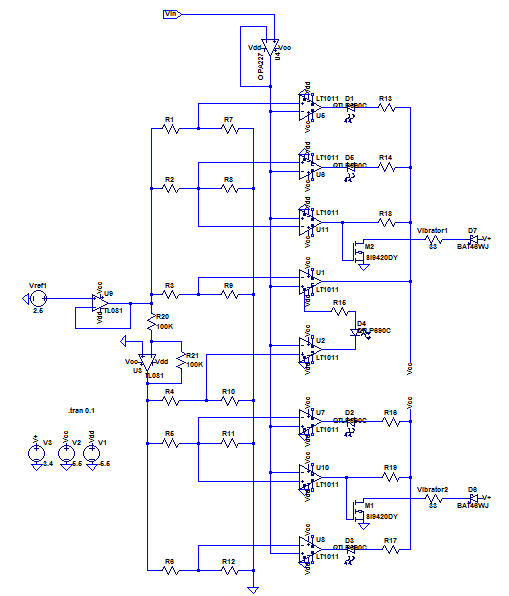
\includegraphics[scale=0.9]{figures/cProblemloesning/komparator_uden_vaerdi.PNG}
	\caption{På figuren ses feedbackkonfigurationen, hvor kredsløbet består af to dele; en for hældning i positiv og negativ retning. Konfigurationen består af otte spændingsdelere bestående af $12$ modstande (R$1$-R$12$) og en spændingsreference. Dertil fem LEDer og vibratorer (i LTspice en modstand) samt tilhørende modstande. For den grønne led, er en vindues-komparatorkonfigurationen  konstrueret vha. komparatorerne (U$3$-U$4$), der anvender en tærskelværdi fra hhv. den negative og positive del af kredsløbet. Kredsløbet er konstrueret i LTspice.}
	\label{fig:komparator_uden_vaerdi}
\end{figure}

%%%%%%%%%%%%%%%%%%%%%%%%%%%%%%%%%%%%%%%%%%%%%%%%%%%%%%%%%%%%%%%

\noindent\textbf{Beregning af tærskelværdier og modstandene R$1$-R$12$ i spændingsdelerne} \\
Det ønskes, at LEDerne skal lyse ved bestemte kropshældninger, dvs. ved bestemte tærskelværdier. Inputsignalet afhænger af den pågældende hældningsgrad, hvilket for komparatoren vil være en bestemt spænding. Komparatorens tærskelværdierne kan beregnes, da værdien i volt pr. grad i hhv. positiv og negativ retning, jævnfør \eqref{taerskelvaerdi_pr_grad} i pilotforsøget i bilag \ref{Pilotforsoeg} på side \pageref{Sec_Pilot_Data}, samt forstærkningsværdien af signalet fra forrige blokke, opsamlings- og tilpasningsblokken, er kendte værdier. Jævnfør tærskelværdierne i afsnit \ref{Komparatorafsnit} på side \pageref{Komparatorafsnit} beregnet ud fra følgende formel:
\begin{eqnarray} \label{pr_grad} 
\text{Tærskelværdi i positiv retning} = {0.0037\text{V}*9.1*3.6*\text{hældningsgrad}} = \text{tærskelværdi} \\
\text{Tærskelværdi i negativ retning} = {0.0036\text{V}*9.1*3.6*\text{hældningsgrad}} = \text{tærskelværdi}
\end{eqnarray}

De udregnede tærskelværdier fremgår af \figref{fig:taerskelvaerdier}. 
\begin{figure}[H]
	\centering
	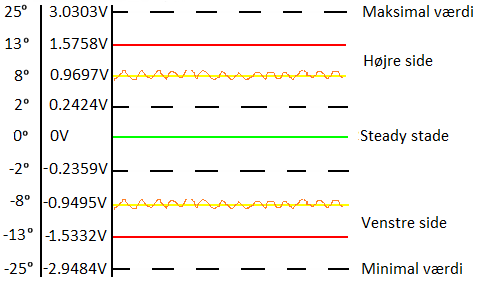
\includegraphics[scale=1.]{figures/cProblemloesning/Taerskelvaerdier.PNG}
	\caption{Af figuren fremgår de beregnede tærskelværdier og hvilket LED, der lyser ved de de enkelte tærskelværdier.}
	\label{fig:taerskelvaerdier}
\end{figure}

\noindent Der anvendes en spændingsreference, bestående af en regulator, der kan levere en konstant spænding på $2.5$V til feedbackkonfigurationen jævnført \ref{subsec:Spaendingsref_Komparator} på side \pageref{subsec:Spaendingsref_Komparator}. Eftersom spændingen ved anvendelse af et batteri vil falde som funktion af tiden benyttes spændingsreferencen, så denne kan holde en fast referencespænding i kredsløbet. Eftersom spændingsreferencen også skal anvendes til de negative tærskelværdier benyttes en inverterende forstærker med et gain på $1$ i designet af feedbackkonfigurationen, hvilket fremgår af figur \figref{fig:komparator_uden_vaerdi}. Ved denne konfiguration vendes signalet, uden at blive forstærket, og kan på denne måde benyttes som referencespænding til negative inputspændinger. For at bestemme R$1$-R$12$ i spændingsdelerne, så LEDerne lyser ved de ønskede tærskelværdier defineres R$1$ til en bestemt værdi. I dette tilfælde fastsættes R$1$ til at være $10$K$\Omega$. Denne værdi er også gældende for R$2$-R$6$, da der benyttes en spændingsdeler for hver tærskelværdi. Derudover er de ønskede tærskelværdier ($V_{out}$) og spændingsreferencen ($V_{in}$) også kendte værdier og R$7$-R$12$ kan dermed udregnes vha. den generelle formel for en spændingsdeler jævnført \eqref{eq:Spaendingsdeler} i afsnit \ref{subsec:Spaendingsref} på side \pageref{subsec:Spaendingsref}. 

\noindent Dette medfører at R$7$-R$12$ giver følgende resultater:\\
R$7$ = $16821\Omega$ \\
R$8$ = $6285\Omega$ \\
R$9$ = $1068\Omega$ \\
R$10$ = $1042\Omega$ \\
R$11$ = $6039\Omega$ \\
R$12$ = $15765\Omega$ \\

%%%%%%%%%%%%%%%%%%%%%%%%%%%%%%%%%%%%%%%%%%%%%%%%%%%%%%%%

\noindent\textbf{Beregning af modstande for den visuelle del af feedbackkonfigurationen} \\
Til den visuelle del af feedbackkonfigurationen anvendes LEDer. En LED har to terminaler; en anode og en katode. Når en ideel LED tændes skyldes det, at der løber strøm fra anoden til katoden og der vil her være et spændingsfald over LEDen på 0V. Dette kaldes fremadgående spænding. Når strømmen løber fra katoden til anoden vil LEDen være slukket, da der ideelt ikke løber strøm igennem kredsløbet.\cite{Sedra2010} Jænvfør kravspecifikationerne i afsnit \ref{KomparatorAfs} på side \pageref{KomparatorAfs} for komparatoren skal forsyningsspændingen være $5.5$V. De anvendte LEDer i systemet er: en grøn L-$53$LG $5$mm (D$3$), to gule L-$53$LY $5$mm (D$2$ og D$4$) og to røde L-$53$LI $5$mm (D$1$ og D$5$). LEDerne kræver en minimum strøm på $2$mA for at lyse og $20$mA hvis de skal give et tydeligt lys.  Spændingsfaldet over LED-dioderne ligger maksimalt i intervallet $2.0$V til $2.2$ V (rød: $2.0$, gul: $2.1$ og grøn: $2.2$), men typisk mellem $1.7$V-$1.9$V. LED-dioderne skal derudover forsynes med $2$mA for at fungere, men kan forsynes op til \fxnote{Tjek og 150mA er rigtigt}$150$mA, før de brændes af. LEDerne forsynes af en $5.5$V spændingsforsyning og tilkobles, som sagt, tilhørende modstande for bla. at undgå at LED-dioderne brænder af. \cite{kingbright} Spændingsfaldet over dioderne samt den spænding LEDerne som minimum skal bruge for at lyse er kendte værdier, dvs. modstandene R$12$-R$17$ kan derfor findes vha. Ohms lov. Nedenstående udregning beregnet en værdi af modstandene, hvis spændingsforsyningen forsyner kredsløbet med $5.5$V og LEDerne med $20$mA for at aktiveres:

%Til den visuelle del af feedbackkonfigurationen anvendes LEDer. En LED har to terminaler; en anode og en katode. Når en ideel LED tændes skyldes det, at der løber strøm fra anoden til katoden og der vil her være et spændingsfald over LEDen på 0V. Dette kaldes fremadgående spændings. Når strømmen løber fra katoden til anoden vil LEDen være slukket, da der ideelt ikke løber strøm igennem kredsløbet. \fxnote{tilføjes mere til teori af LED}
%Jænvfør kravspecifikationerne i afsnit \ref{KomparatorAfs} på side \pageref{KomparatorAfs} for komparatoren skal forsyningsspændingen være $5.5$V. De anvendte LEDer i systemet er: en grøn L-$53$LG $5$mm (D$3$), to gule L-$53$LY $5$mm (D$2$ og D$4$) og to røde L-$53$LI $5$mm (D$1$ og D$5$). LEDerne kræver en minimum strøm på $2$mA for at lyse og $20$mA hvis de skal give et tydeligt lys.  Spændingsfaldet over LED-dioderne ligger maksimalt i intervallet $2.0$V til $2.2$ V (rød: $2.0$, gul: $2.1$ og grøn: $2.2$), men typisk mellem $1.7$V-$1.9$V. LED-dioderne skal derudover forsynes med $2$mA for at fungere, men kan forsynes op til \fxnote{Tjek og 150mA er rigtigt}$150$mA, før de brændes af. LEDerne forsynes af en $5.5$V spændingsforsyning og tilkobles, som sagt, tilhørende modstande for bla. at undgå at LED-dioderne brænder af. \cite{kingbright} Spændingsfaldet over dioderne samt den spænding LEDerne som minimum skal bruge for at lyse er kendte værdier, dvs. modstandene R$12$-R$17$ kan derfor findes vha. Ohms lov. Nedenstående udregning beregnet en værdi af modstandene, hvis spændingsforsyningen forsyner kredsløbet med $5.5$V og LEDernes med $20$mA for at aktiveres:

\begin{equation}
R = \dfrac{5.5V - 2.2V}{0.02A} = 165\Omega
\end{equation}
\noindent Dermed sættes modstandene R$13$-R$14$, R$16$-R$17$ og R$19$ til $165\Omega$ for at sikre, at der er $20$mA til LEDerne, så de kan give et tydeligt lys og derudover sørge for, at der ikke er for meget strøm i kredsløbet, så batterierne drænes. 

%%%%%%%%%%%%%%%%%%%%%%%%%%%%%%%%%%%%%%%%%%%%%%%%%%%%%%%%%%%

\noindent\textbf{Beregning af modstande for den somasensoriske del af feedbackkonfigurationen} \\
Til den somasensoriske del af feedbackkonfigurationen benyttes vibratorer, jævnført \ref{KomparatorAfs} på side \pageref{KomparatorAfs}. En vibrator er en elektrisk motor, der skaber svingninger, hvilket medfører en vibration.\cite{Radaktionen2009}. Vibratorerne der anvendes er af typen C1026B. Den har et drift arbejdsområde på $2.7-3.3$V, der typisk ligger på $3$V og starter ved $2.3$V. Vibratorerne skal derfor have en spændingsforsyning på $3$V. Derudover er startstørmmen $120$mA, og når motoren kører er driftstrømmen på $90$mA. Herefter sker vibrationen med en frekvens på $10-55$Hz, afhængig af spændingsforsyningen, samt strømmen i kredsløbet. \cite{Machinery2009} Jævnfør kravspecifikationerne benyttes vibratorer med dimensionerne; $1$cm i diameter og $0.27$cm i tykkelse, så de kan påsættes patienternes hænder. 
 
For at opnå et tilstrækkeligt strømniveau anvendes en transistor af typen; BS$170$ for at generere en større mængde strøm i kredsløbet. Transistoren placeres mellem vibratoren og komparatoren. Det er designet således, at transistoren tændes og vibratoren aktiveres, når komparatoren er slukket, modsat komparatorerne, der benyttes i forbindelse med LEDerne. Dette skyldes, at når komparatoren er tændt vil den trække spænding tilkoblet et knudepunkt mellem komparatorens collector-terminal og trasistorens gain-terminal. Modstandene R$15$ og R$18$ er placeret ved spændingsforsyningen på $5.5$V ($+V_{cc}$) og bestemmes til at være $100$K. Disse skal sørge for at kredsløbet ikke bruger for meget strøm, hvorfor der er valgt modstande med en høj værdi. Når komparatoren slukker vil spændingen aktivere transistoren og der dannes forbindelse mellem transistorens drain- og source-terminal. Dette vil aktivere vibratorerne. Spændingsforsyningen til vibratorerne er på $3.4$V ($V+$) og forsynes af spændingsregulatoren. Eftersom vibratoren kun skal forsynes med $3$V benyttes en schottky-diode (BAT$41$), der nedsætter spændingen til under $3$V. Schottky-dioden fungerer således, at der sker et spændingsfald afhængig af strømmen, der løber igennem dioden. Spændingsforsyningen på $3.4$V aktiveres, når komparatoren slukker og der er forbindelse mellem transistorens drain- og source-terminal, da strømmen kan løbe til ground i source-terminalen. Den somasensoriske del af feedbackkonfigurationen fremgår af \figref{$fig:komparator_uden_vaerdi$}.
 
\subsubsection{Simulering}
Den visuelle og somatosensoriske del af feedbackkonfigurationen simuleres med et sinus-signal, der svinger mellem $\pm3$V.\fxnote{skal vi skrive Vpp?} Dette gøres for at simulere signalet, der kommer fra den forrige blok, som har et arbejdsområde på $\pm3$V. I simuleringen testes, hvorvidt tærskelværdierne kan accepteres ift. kravspecifikationer. Kredsløbet simuleres ikke med en spændingsreference, men derimod en spændingsforsyning på $2.5$V, der indikerer spændingsreferencen. Af figur \figref{fig:komparator_samlet} fremgår hele feedbackkonfigurationen, der simuleres i LTspice.

\begin{figure}[H]
	\centering
	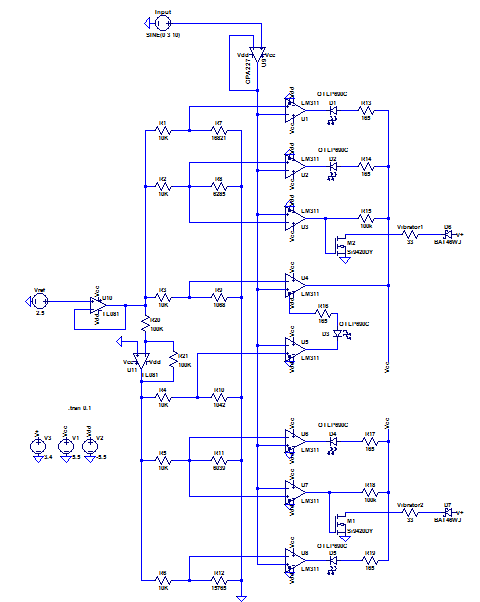
\includegraphics[scale=0.9]{figures/cProblemloesning/komparator_samlet.PNG}
	\caption{Af figuren fremgår feedbackkonfigurationen med beregnede modstande. Kredsløbet simuleres i LTspice vha. et sinus-signal, der svinger mellem $\pm3$V.}
	\label{fig:komparator_samlet}
\end{figure}
 
\noindent\textbf{Simulering af den visuelle del af feedbackkonfigurationen} \\
Til simulering af den visuelle den af feedbackkonfiguration anvendes komparatorer af typen LM$311$ og LEDer af typen QTLP$690$C, da de reelle komponenter ikke kan vælges i LTspice.\fxnote{skal vi slette det med LM311?} Kredsløbet simuleres i LTspice for at teste, hvorvidt den visuelle del af feedbackkonfiguration opfylder de opstillede kravspecifikationer, jævnfør afsnit \ref{KomparatorAfs} på side \pageref{KomparatorAfs}. Af \figref{fig:komparator_visuel_simulering_samlet1} fremgår tærskelværdierne for den visuelle del af feedbackkonfigurationen. 

\begin{figure}[H]
	\centering
	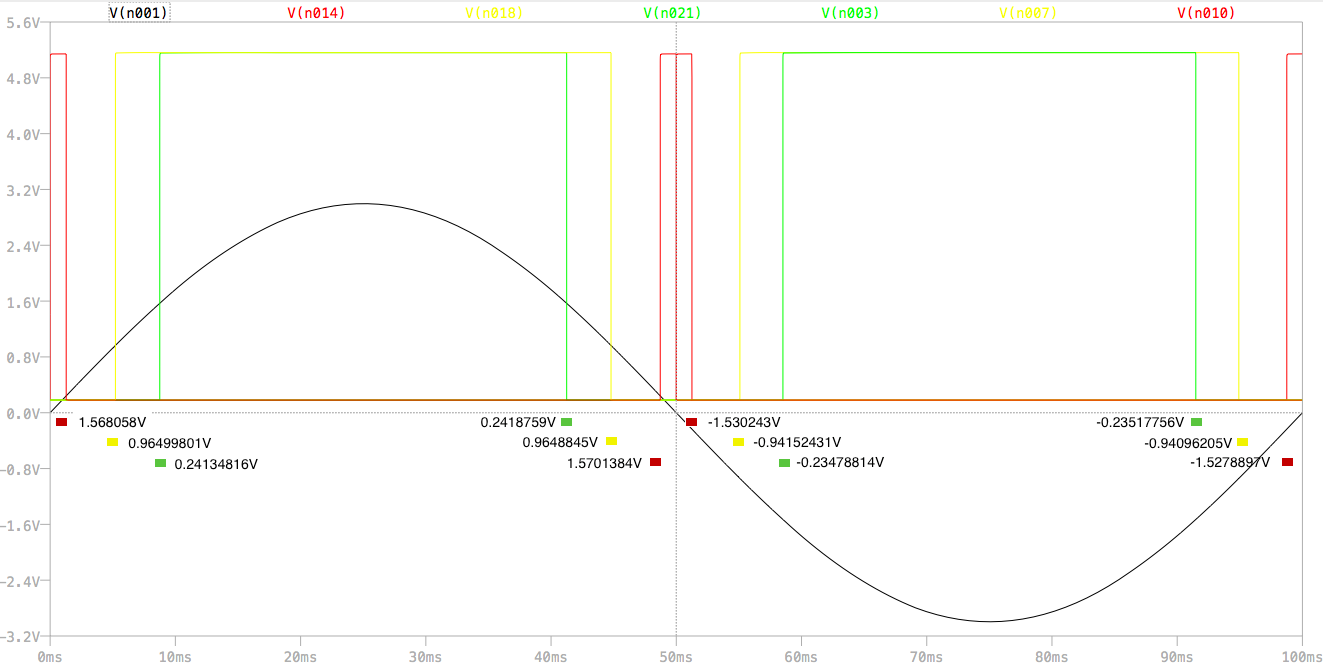
\includegraphics[scale=0.3]{figures/cProblemloesning/komparator_visuel_simulering_samlet1.PNG}
	\caption{På figuren ses simuleringen af den visuelle del af feedbackkonfiguration. V(n$002$) er sinus-signalet, der illustrerer blokkens inputsignal, V(n$004$) viser spændingsfaldet for de røde LEDer, V(n$008$) for de gule LEDer og V(n$015$) for den grønne LED. Når inputsignalet når de definerede tærskelværdier, vil kurverne gå i negativ mætning og LED-dioderne vil lyse. Kredsløbet er simuleret i LTspice.}
	\label{fig:komparator_visuel_simulering_samlet1}
\end{figure}

\noindent På \figref{fig:komparator_visuel_simulering_samlet1} fremgår det, at ved de enkelte tærskelværdier går signalet i negativ mætning, hvilket får LED-dioderne til at lyse. Afvigelsen mellem det teoretiske og simulerede reference input beregnes og vil fremgå af \ref{Tab:test_reference}

\begin{table}[H]
	\centering
	\begin{tabular}{|l|l|l|l|} \hline
		& \textit{\begin{tabular}[c]{@{}l@{}}Teoretisk\\ reference\\ input\end{tabular}} & \textit{\begin{tabular}[c]{@{}l@{}}Simuleret\\ reference\\ input\end{tabular}} & \textit{\% afvigelse} \\ \hline
		\textit{$13^{\circ}$}  & $1.5758$V                                                                      & $1.5659$V                                                                  & $0.63\%$              \\ \hline
		\textit{$8^{\circ}$}   & $0.9697$V                                                                      & $0.9654$V                                                                  & $0.44\%$              \\ \hline
		\textit{$2^{\circ}$}   & $0.2424$V                                                                      & $0.2415$V                                                                  & $0.37\%$              \\ \hline
		\textit{-$2^{\circ}$}  & -$0.2359$V                                                                     & -$0.2348$V                                                                 & $0.47\%$              \\ \hline
		\textit{-$8^{\circ}$}  & -$0.9495$V                                                                     & -$0.9341$V                                                                 & $0.92\%$              \\ \hline
		\textit{-$13^{\circ}$} & -$1.5332$V                                                                     & -$1.5320$V                                                                 & $0.08\%$        \\ \hline     
	\end{tabular}
	\caption{Af tabelle fremgår de teoretiske og simulerede tærskelværdier ved de enkelte hældningsgrader, samt afvigelsen mellem disse.}
	\label{Tab:test_reference1}
\end{table}

%\begin{table}[H]
%	\centering
%	\begin{tabular}{|l|l|l|l|l|l|}
%		\hline
%					& \textit{Tærskelværdier} 	& \textit{Måling til højre} & \textit{Måling til venstre}		&  \textit{\begin{tabular}[c]{@{}l@{}}Afvigelse\\ for højre\end{tabular}}   &  \textit{\begin{tabular}[c]{@{}l@{}}Afvigelse\\ for venstre\end{tabular}}   \\ \hline
%\textbf{$2^{\circ}$} 		& $0.2412$V  				&$0.23815127$V 			&$-0.17571651$V		& $1.3\%$  &$??\%$ \\ \hline
% \textbf{$8^{\circ}$} 		&$0.9648$V					&$0.96551609$V			&$0.96777598$V		& $0.07\%$	&$0.3\%$\\ \hline
%\textbf{-$8^{\circ}$} 		&-$0.9413$V					&-$0.96784376$V 			&-$0.92251539$V		& $2.8\%$	&$2\%$\\ \hline 		
%\textbf{$13^{\circ}$} 		&$1.5679$V 					&$1.5583895$V 		  	&$1.5705552$V		& $0.6\%$	&$0.2\%$\\ \hline
%\textbf{-$13^{\circ}$} 		&-$1.5297$VV 				&-$1.5297296$V		   	&-$1.5297259$V		& $0.002\%$	&$0.002\%$ \\ \hline
%	\end{tabular}
%	\caption{I tabellen ses der, at de anvendte tærskelværdier afviger fra den teoretiske værdi, hvilket er forventet af reelle komponenter. Det er en acceptabel afvigelse, så tærskelværdierne kan derfor anvendes til implementering}
%	\label{Tab:Maalingtearskelvaerdier}
%\end{table}

\noindent Det kan udfra \ref{Tab:test_reference1} konkluderes, at afvigelsen fra de udregnede tærskelværdier stemmer overens med tolerancekravene for komparatorens tærkselværdier, jævnfør afsnit \ref{KomparatorAfs} på side \pageref{KomparatorAfs}, hvorfor den visuelle del af feedbackkonfigurationen accepteres. 

\noindent\textbf{Simulering af somatosensoriske del af feedbackkonfigurationen} \\
Til simulering af den somatosensoriske del af feedbackkonfigurationen anvendes komparatorer af typen LM$311$ og da der ikke findes vibratorer i LTspice benyttes en modstand på R$33$ udregnet vha. Ohms lov, hvilket fremgår af nedestående \eqref{vibrator_modstand} 

\begin{equation} \label{vibrator_modstand}
R = \dfrac{3V}{0.9A} = 33\Omega
\end{equation}

\noindent Kredsløbet simuleres i LTspice for at teste, hvorvidt den somatosensoriske del af feedbackkonfiguration opfylder kravspecifikationerne, jævnfør afsnit \ref{KomparatorAfs} på side \pageref{KomparatorAfs}. Af figur \figref{fig:vibration_graf} fremgår tærskelværdierne for den visuelle del af feedbackkonfigurationen.

\begin{figure}[H]
	\centering
	\includegraphics[scale=0.3]{figures/cProblemloesning/vibration_graf.PNG}
	\caption{På figuren ses simuleringen af den somatosensoriske del af feedbackkonfiguration. V(n$002$ er sinus-signalet, der illustrerer blokkens inputsignal. I(D$6$) og I(D$7$) er tærskelværdien for hhv. den højre og venstre vibrator. Kredsløbet er simuleret i LTspice.}
	\label{fig:vibration_graf}
\end{figure}
\noindent På \figref{fig:vibration_graf} fremgår det, at ved de enkelte tærskelværdier går signalet i negativ mætning, hvilket aktiverer vibratorerne. Derudover fremgår det af figuren, at tærskelværdier for de to vibratorer er de samme tærskelværdier for den gule LED, hvilket gør, at den samme afvigelse vil gøre sig gældende, hvorfor den somatosensoriske del af feedbackkonfigurationen accepteres. 

\subsubsection{Implementering og test}
Ifølge det valgte design benyttes i alt 21 modstande antal modstande. Ved reelle komponenter vil der være en afvigelse, hvilket fremgår af tabel \ref{Tab:komparator_modstande}. Derudover er det ikke muligt at anvende alle beregnede komponenter, hvorfor der anvendes modstande i serie- og parallelforbindelser. I tabellen vil alle modstandene fremgå, samt den afvigelsen mellem den teoretiske og målte modstand. 
\begin{table}[H]
\centering
\begin{tabular}{|l|l|l|l|}
\hline
\textit{}               & \textit{Teoretisk værdi} & \textit{Målt værdi} & \textit{Afvigelse} \\ \hline
\textit{R1}             & $10$K$\Omega$            & $9.973$K$\Omega$    & $0.27\%$           \\ \hline
\textit{R2}             & $10$K$\Omega$            & $9.992$K$\Omega$    & $0.08\%$           \\ \hline
\textit{R3}             & $10$K$\Omega$            & $9.976$K$\Omega$    & $0.24\%$           \\ \hline
\textit{R4}             & $10$K$\Omega$            & $9.950$K$\Omega$    & $0.50\%$           \\ \hline
\textit{R5}             & $10$K$\Omega$            & $9.985$K$\Omega$    & $0.15\%$           \\ \hline
\textit{R6}             & $10$K$\Omega$            & $9.950$K$\Omega$    & $0.50\%$           \\ \hline
\textit{R7 (Serie)}     & $16.821$K$\Omega$        & $16.758$K$\Omega$   & $0.37\%$           \\ \hline
\textit{R8 (Parallel)}  & $6.285$K$\Omega$         & $6.280$K$\Omega$    & $0.08\%$           \\ \hline
\textit{R9 (Serie)}     & $1068\Omega$             & $1065\Omega$        & $0.28\%$           \\ \hline
\textit{R10 (Serie)}    & $1042\Omega$             & $1036\Omega$        & $0.58\%$           \\ \hline
\textit{R11 (Parallel)} & $6.039$K$\Omega$         & $6.044$K$\Omega$    & $0.08\%$           \\ \hline
\textit{R12 (Parallel)} & $15.765$K$\Omega$        & $15.718$K$\Omega$   & $0.30\%$           \\ \hline
\textit{R13 (Serie)}    & $165\Omega$              & $164.59\Omega$      & $0.25\%$           \\ \hline
\textit{R14 (Serie)}    & $165\Omega$              & $164.54\Omega$      & $0.28\%$           \\ \hline
\textit{R15}            & $100$K$\Omega$           & $99.660$K$\Omega$   & $0.34\%$           \\ \hline
\textit{R16 (serie)}    & $165\Omega$              & $164.87\Omega$      & $0.08\%$           \\ \hline
\textit{R17 (Serie)}    & $165\Omega$              & $165.07\Omega$      & $0.04\%$           \\ \hline
\textit{R18}            & $100$K$\Omega$           & $99.722$K$\Omega$   & $0.28\%$           \\ \hline
\textit{R19 (Serie)}    & $165\Omega$              & $163.90\Omega$      & $0.67\%$           \\ \hline
\textit{R20}            & $100$K$\Omega$           & $99.628$K$\Omega$   & $0.37\%$           \\ \hline
\textit{R21}            & $100$K$\Omega$           & $99.676$K$\Omega$   & $0.32\%$           \\ \hline
\end{tabular}
\caption{Af tabellen fremgår de teoretiske og reelle værdier for modstandene benyttet i feedbackkonfigurationen.}
\label{Tab:komparator_modstande}
\end{table}
\noindent Komparatorkonfigurationen testes ved en spændingsforsyning på $5.5$V med et sinussignal som input. Af \ref{Tab: test_reference} fremgår de beregnede og målte tærskelværdier, samt afvigelsen af disse tærskelværdier. 

\begin{table}[H]
	\centering
	\begin{tabular}{|l|l|l|l|} \hline
		& \textit{\begin{tabular}[c]{@{}l@{}}Teoretisk\\ reference\\ input\end{tabular}} & \textit{\begin{tabular}[c]{@{}l@{}}Målte\\ reference\\ input\end{tabular}} & \textit{\% afvigelse} \\ \hline
		\textit{$13^{\circ}$}  & $1.5758$V                                                                      & $1.5748$V                                                                  & $0.06\%$              \\ \hline
		\textit{$8^{\circ}$}   & $0.9697$V                                                                      & $0.9700$V                                                                  & $0.31\%$              \\ \hline
		\textit{$2^{\circ}$}   & $0.2424$V                                                                      & $0.2427$V                                                                  & $0.12\%$              \\ \hline
		\textit{-$2^{\circ}$}  & -$0.2359$V                                                                     & -$0.2373$V                                                                 & $0.59\%$              \\ \hline
		\textit{-$8^{\circ}$}  & -$0.9495$V                                                                     & -$0.9492$V                                                                 & $0.03\%$              \\ \hline
		\textit{-$13^{\circ}$} & -$1.5332$V                                                                     & -$1.5418$V                                                                 & $0.56\%$        \\ \hline     
	\end{tabular}
	\caption{Af tabellen fremgår de teoretiske og målte tærskelværdier ved de enkelte hældningsgrader, samt afvigelsen mellem disse tærskelværdier.}
	\label{Tab:test_reference}
\end{table}
\noindent Jævnfør kravspecifikationerne afsnit \ref{KomparatorAfs} på side \pageref{KomparatorAfs} overholder de målte tærskelværdier tolerancekravet på $\pm1\%$. For at undersøge, hvornår LEDerne og vibratorerne tænder og slukker måles på input- og outputsignalet vha. et osciolloskop. I \tableref{Tab:test-taendsluk} fremgår de teoretiske og målte tærskelværdier for hvornår LEDen og vibratorerne tænder og slukker, samt afvigelsen mellem disse tærskelværdier. 

%\begin{table}[H]
%\centering
%\begin{tabular}{|l|l|l|l|l|l|l|}
%\hline
%                    & \textit{Målt reference input} & \textit{Målt Tænd}     & \textit{Afvigelse}      & %\textit{Teoretisk sluk}              & \textit{Målt sluk}  & \textit{Afvigelse}      \\ \hline
%\textit{$13\circ$}  & $<1.5758$V              & $1.6000$V              & $1.5357\%$               & $>1.5758$                            & $1.6000$V           & $1.5357$                \\ \hline
%\textit{$8\circ$}   & $<0.9697$V              & $1.0000$V              & $3.1246\%$               & $>0.9697$V                           & $0.9600$V           & $1.0000\%$               \\ \hline
%\textit{$0\circ$}   & -$0.2359 - 0.2424$      & \begin{tabular}[c]{@{}l@{}} -$0.2400$\\ og $0.2800$V\end{tabular} & \begin{tabular}[c]{@{}l@{}}$1.7380\%$\\ og $15.5115\%$\end{tabular} & \begin{tabular}[c]{@{}l@{}}<-$0.2359$\\ og $\textgreater0.2424\%$\end{tabular} & \begin{tabular}[c]{@{}l@{}}-$0.240$\\ og $0.280$\end{tabular} & \begin{tabular}[c]{@{}l@{}}$1.7380\%$\\ og $15.5115\%$\end{tabular} \\ \hline
%\textit{-$8\circ$}  & $<$-$0.9495$V           & -$0.9200$V             & $3.1069\%$               & $>$-$0.9495$V                        & -$0.9200$V          & $3.1069\%$               \\ \hline
%\textit{-$13\circ$} & $<$-$1.5332$V           & -$1.5300$V             & $0.2087\%$               & $>$-$1.5332$V                        & -$1.5400$V          & $0.4435\%$               \\ \hline
%\end{tabular}
%\caption{Af tabellen fremgår det, hvornår LEDerne teoretisk bør slukke og tænde og hvornår de blev målt til at tænde og slukke.}
%\label{Tab:test-taendsluk}
%\end{table}

\begin{table}[H]
\centering
\begin{tabular}{|l|l|l|l|}
\hline
           & \textit{Målte reference input} & \textit{Målt reference output} & \textit{\% afvigelse} \\ \hline
$13\circ$  & $1.5748$V                      & $1.5600$V                      & $1.14$ \%              \\ \hline
$8\circ$   & $0.9700$V                      & $1.000$V                       & $3.09$ \%              \\ \hline
$2\circ$   & $0.2427$V                      & $0.2400$V                      & $1.11$ \%                                    \\ \hline
-$2\circ$  & -$0.2373$V                     & -$0.2000$V                     & $15.72$ \%                                \\ \hline
-$8\circ$  & -$0.9492$V                     & -$0.9200$V                     & $3.18$ \%              \\ \hline
-$13\circ$ & -$1.5418$V                     & $1.5200$V                      & $1.44$ \%              \\ \hline
\end{tabular}
\caption{Af tabellen fremgår de målte reference input og output, samt afvigelsen af disse værdier. Derudover er afvigelsen regnet ud i grader.}
\label{Tab:test-taendsluk}
\end{table}

\noindent De målte reference output blev målt vha. et osciolloskop, der har en 8-bits ADC-konverter \cite{RIGOL2010}. Under testen blev det observeret, at Y-aksen (volt) ændres med $0.04$V pr. målepunkt og idet tærskelværdierne kunne være placeret mellem to målepunkter var ikke muligt at aflæse det præcise reference input og output. Af \ref{Tab:test-taendsluk} fremgår den beregnede afvigelse mellem den målte reference input og output, samt hvad denne afvigelse er i grader. Jævnfør kravspecifikationerne afsnit \ref{KomparatorAfs} på side \pageref{KomparatorAfs} ligger afvigelsen indenfor tolerancekravene, hvorfor afvigelserne i tabellen accepteres. 